% answers.tex —— 2010 年·普通高等学校招生考试·天津卷·理科 · 参考答案与详细解析片段
% 由 tools/generate_projects.py 依来源总账自 2010/2010_数学真题_天津理_试题.md + 2010/2010_数学真题_天津理_解析正文.md + 2010/2010_数学真题_天津理_答案要点.md 生成，勿手改（改源 MD 后重跑）


\begin{gktip}
固定候选 PDF 仅含题面，无答案、解析和评分标准，原页亦未标分值；以下为非官方编者独立推导，官方答案字段为空。分数、根号、上下标与六幅图均以 600 dpi 原页复核。
\end{gktip}

\begin{answer}
\gksolhead{1}{}

\textbf{题目}：

$i$ 是虚数单位，复数 $\dfrac{-1+3i}{1+2i}=$（　）

（A）$1+i$

（B）$5+5i$

（C）$-5-5i$

（D）$-1-i$

\Needspace{4\baselineskip}
\textbf{解析}

\Needspace{5\baselineskip}
把分子、分母同乘 $1-2i$。

\nopagebreak[4]
\[\frac{-1+3i}{1+2i}=\frac{(-1+3i)(1-2i)}{(1+2i)(1-2i)}
=\frac{5+5i}5=1+i.\]

故选 A。

\gkanswer{答案：A。}

\end{answer}
\begin{answer}
\gksolhead{2}{}

\textbf{题目}：

函数 $f(x)=2^x+3x$ 的零点所在的一个区间是（　）

（A）$(-2,-1)$

（B）$(-1,0)$

（C）$(0,1)$

（D）$(1,2)$

\Needspace{4\baselineskip}
\textbf{解析}

计算区间端点的函数值。

$f(-1)=\dfrac12-3<0$，$f(0)=1>0$，且 $f$ 在 $\mathbf R$ 上单调递增，故零点在 $(-1,0)$。选 B。

\gkanswer{答案：B。}

\end{answer}
\begin{answer}
\gksolhead{3}{}

\textbf{题目}：

命题“若 $f(x)$ 是奇函数，则 $f(-x)$ 是奇函数”的否命题是（　）

（A）若 $f(x)$ 是偶函数，则 $f(-x)$ 是偶函数

（B）若 $f(x)$ 不是奇函数，则 $f(-x)$ 不是奇函数

（C）若 $f(-x)$ 是奇函数，则 $f(x)$ 是奇函数

（D）若 $f(-x)$ 不是奇函数，则 $f(x)$ 不是奇函数

\Needspace{4\baselineskip}
\textbf{解析}

否命题要同时否定条件与结论，且不交换条件与结论。

原命题的条件是“$f(x)$ 是奇函数”，结论是“$f(-x)$ 是奇函数”，故否命题为“若 $f(x)$ 不是奇函数，则 $f(-x)$ 不是奇函数”。选 B。

\gkanswer{答案：B。}

\end{answer}
\begin{answer}
\gksolhead{4}{}

\textbf{题目}：

阅读下面的程序框图，若输出 $s$ 的值为 $-7$，则判断框内可填写（　）
\nopagebreak[4]
\begin{center}% 2010 年天津卷理科第 4 题：程序框图，输出 s = −7 时判断框内的条件。
% 来源 PDF：普通高考/2010/2010天津理.pdf，SHA-256 340aba76699a12f330637f9c682abbc893e03e0e91788287934c0a7e0a3cace9。
% 原页：第 1 页（A3 六栏）第 1 栏中部，书页码 635。
% 重绘依据：开始 → i=1 → s=2 → 判断；是（左）→ s=s−i → i=i+2 → 回到判断前的竖线；
%   否（下）→ 输出 s → 结束。原页判断框内为空。
\begin{tikzpicture}[semithick, >=Stealth,
  every node/.style={inner sep=2pt, font=\small}, node distance=5mm]
  \node (start) [draw, rounded corners=4pt, minimum width=2cm, minimum height=0.55cm] {开始};
  \node (i1) [draw, minimum width=1.6cm, minimum height=0.55cm, below=of start] {$i=1$};
  \node (s2) [draw, minimum width=1.6cm, minimum height=0.55cm, below=of i1] {$s=2$};
  \node (cond) [draw, diamond, aspect=2.2, minimum width=3cm,
    minimum height=1.1cm, below=16mm of s2] {};
  \node (out) [draw, trapezium, trapezium left angle=72, trapezium right angle=108,
    minimum width=2.4cm, minimum height=0.55cm, below=9mm of cond] {输出 $s$};
  \node (end) [draw, rounded corners=4pt, minimum width=2cm, minimum height=0.55cm,
    below=of out] {结束};
  \node (ss) [draw, minimum width=2.6cm, minimum height=0.55cm,
    left=13mm of cond] {$s=s-i$};
  \node (ii) [draw, minimum width=2.6cm, minimum height=0.55cm,
    above=6mm of ss] {$i=i+2$};

  \draw[->] (start) -- (i1);
  \draw[->] (i1) -- (s2);
  \draw[->] (s2) -- (cond);
  \draw[->] (cond) -- node[right] {否} (out);
  \draw[->] (out) -- (end);
  \draw[->] (cond.west) -- node[above, pos=0.72] {是} (ss.east);
  \draw[->] (ss.north) -- (ii.south);
  \draw (ii.north) -- ++(0,0.35) -| ($(s2.south)!0.5!(cond.north)$);
\end{tikzpicture}
\end{center}
\nopagebreak[4]
（A）$i<3?$

（B）$i<4?$

（C）$i<5?$

（D）$i<6?$

\Needspace{4\baselineskip}
\textbf{解析}

按框图，先判断条件，再执行 $s=s-i$ 与 $i=i+2$。

\Needspace{5\baselineskip}
取 $i<6?$ 时：

\nopagebreak[4]
\[i=1:\ s=2-1=1,\ i=3;\qquad i=3:\ s=1-3=-2,\ i=5;\]

\nopagebreak[4]
\[i=5:\ s=-2-5=-7,\ i=7.\]

此时 $7<6$ 不成立，输出 $s=-7$。逐一检验其余条件：$i<3?$ 输出 $1$，$i<4?$ 与 $i<5?$ 都输出 $-2$，均不合题意。选 D。

\gkanswer{答案：D。}

\end{answer}
\begin{answer}
\gksolhead{5}{}

\textbf{题目}：

已知双曲线 $\dfrac{x^2}{a^2}-\dfrac{y^2}{b^2}=1$（$a>0$，$b>0$）的一条渐近线方程是 $y=\sqrt3x$，它的一个焦点在抛物线 $y^2=24x$ 的准线上，则双曲线的方程为（　）

（A）$\frac{x^2}{36}-\frac{y^2}{108}=1$

（B）$\frac{x^2}9-\frac{y^2}{27}=1$

（C）$\frac{x^2}{108}-\frac{y^2}{36}=1$

（D）$\frac{x^2}{27}-\frac{y^2}9=1$

\Needspace{4\baselineskip}
\textbf{解析}

由渐近线先定 $a$、$b$ 的比例，再由准线定 $c$。

\Needspace{5\baselineskip}
渐近线 $y=\sqrt3x$ 给出 $\dfrac ba=\sqrt3$。抛物线 $y^2=24x$ 的准线为 $x=-6$，故双曲线的一个焦点为 $(-6,0)$，$c=6$。由

\nopagebreak[4]
\[c^2=a^2+b^2=4a^2=36\]

得 $a^2=9$，$b^2=27$，双曲线为 $\dfrac{x^2}9-\dfrac{y^2}{27}=1$。选 B。

\gkanswer{答案：B。}

\end{answer}
\begin{answer}
\gksolhead{6}{}

\textbf{题目}：

已知 $\{a_n\}$ 是首项为 $1$ 的等比数列，$S_n$ 是 $\{a_n\}$ 的前 $n$ 项和，且 $9S_3=S_6$。

则数列 $\left\{\dfrac1{a_n}\right\}$ 的前 $5$ 项和为（　）

（A）$\frac{15}8$ 或 $5$

（B）$\frac{31}{16}$ 或 $5$

（C）$\frac{31}{16}$

（D）$\frac{15}8$

\Needspace{4\baselineskip}
\textbf{解析}

设公比为 $q$，用 $S_6=S_3(1+q^3)$ 求 $q$。

\Needspace{5\baselineskip}
由 $9S_3=S_6$ 得

\nopagebreak[4]
\[9S_3=S_3(1+q^3)\Longrightarrow q^3=8,\ q=2.\]

\Needspace{5\baselineskip}
于是 $\left\{\dfrac1{a_n}\right\}$ 是首项 $1$、公比 $\dfrac12$ 的等比数列，前 $5$ 项和为

\nopagebreak[4]
\[S=\frac{1-\left(\frac12\right)^5}{1-\frac12}=\frac{31}{16}.\]

选 C。

\gkanswer{答案：C。}

\end{answer}
\begin{answer}
\gksolhead{7}{}

\textbf{题目}：

在 $\triangle ABC$ 中，内角 $A$，$B$，$C$ 的对边分别是 $a$，$b$，$c$，若 $a^2-b^2=\sqrt3bc$，$\sin C=2\sqrt3\sin B$，则 $A=$（　）

（A）$30^\circ$

（B）$60^\circ$

（C）$120^\circ$

（D）$150^\circ$

\Needspace{4\baselineskip}
\textbf{解析}

先用正弦定理把角的条件化为边的条件。

\Needspace{5\baselineskip}
由 $\sin C=2\sqrt3\sin B$ 得 $c=2\sqrt3b$。代入 $a^2-b^2=\sqrt3bc$ 得

\nopagebreak[4]
\[a^2=b^2+\sqrt3\cdot b\cdot2\sqrt3b=7b^2.\]

\Needspace{5\baselineskip}
故

\nopagebreak[4]
\[\cos A=\frac{b^2+c^2-a^2}{2bc}
=\frac{b^2+12b^2-7b^2}{4\sqrt3b^2}=\frac{\sqrt3}2,\]

所以 $A=30^\circ$。选 A。

\gkanswer{答案：A。}

\end{answer}
\begin{answer}
\gksolhead{8}{}

\textbf{题目}：

设函数 $f(x)=\begin{cases}\log_2x,&x>0,\\ \log_{\frac12}(-x),&x<0,\end{cases}$ 若 $f(a)>f(-a)$，则实数 $a$ 的取值范围是（　）

（A）$(-1,0)\cup(0,1)$

（B）$(-\infty,-1)\cup(1,+\infty)$

（C）$(-1,0)\cup(1,+\infty)$

（D）$(-\infty,-1)\cup(0,1)$

\Needspace{4\baselineskip}
\textbf{解析}

按 $a>0$ 与 $a<0$ 分别去绝对值与对数符号。

当 $a>0$ 时，$f(a)=\log_2a$，$f(-a)=\log_{\frac12}a=-\log_2a$，不等式化为 $2\log_2a>0$，得 $a>1$。

当 $a<0$ 时，$f(a)=\log_{\frac12}(-a)$，$f(-a)=\log_2(-a)$，不等式化为 $-\log_2(-a)>\log_2(-a)$，即 $\log_2(-a)<0$，得 $0<-a<1$，即 $-1<a<0$。

故 $a\in(-1,0)\cup(1,+\infty)$。选 C。

\gkanswer{答案：C。}

\end{answer}
\begin{answer}
\gksolhead{9}{}

\textbf{题目}：

设集合 $A=\{x\mid|x-a|<1,x\in\mathbf R\}$，$B=\{x\mid|x-b|>2,x\in\mathbf R\}$。若 $A\subseteq B$，则实数 $a$，$b$ 必满足（　）

（A）$|a+b|\leqslant3$

（B）$|a+b|\geqslant3$

（C）$|a-b|\leqslant3$

（D）$|a-b|\geqslant3$

\Needspace{4\baselineskip}
\textbf{解析}

把两个集合都写成区间。

\Needspace{5\baselineskip}
$A=(a-1,a+1)$，$B=(-\infty,b-2)\cup(b+2,+\infty)$。$A\subseteq B$ 等价于

\nopagebreak[4]
\[a+1\leqslant b-2\quad\text{\text{或}}\quad a-1\geqslant b+2,\]

即 $b-a\geqslant3$ 或 $a-b\geqslant3$，也就是 $|a-b|\geqslant3$。选 D。

\gkanswer{答案：D。}

\end{answer}
\begin{answer}
\gksolhead{10}{}

\textbf{题目}：

如图，用四种不同颜色给图中的 $A$，$B$，$C$，$D$，$E$，$F$ 六个点涂色，要求每个点涂一种颜色，且图中每条线段的两个端点涂不同颜色，则不同的涂色方法有（　）
\nopagebreak[4]
\begin{center}% 2010 年天津卷理科第 10 题：矩形 ABCD 与两个内点 E、F 的涂色图。
% 来源 PDF：普通高考/2010/2010天津理.pdf，SHA-256 340aba76699a12f330637f9c682abbc893e03e0e91788287934c0a7e0a3cace9。
% 原页：第 1 页（A3 六栏）第 2 栏中部，书页码 635。
% 重绘依据：矩形 ABCD（A 左上、D 右上、B 左下、C 右下），E 在上部与 A、D 相连，
%   F 在下部与 B、C 相连，E 与 F 相连；无矩形的对角线。
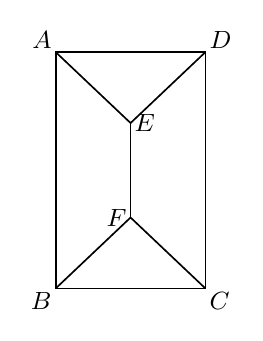
\begin{tikzpicture}[semithick, every node/.style={inner sep=1.2pt, font=\small}]
  \coordinate (A) at (0,3);
  \coordinate (D) at (1.9,3);
  \coordinate (B) at (0,0);
  \coordinate (C) at (1.9,0);
  \coordinate (E) at (0.95,2.1);
  \coordinate (F) at (0.95,0.9);
  \draw (A) -- (D) -- (C) -- (B) -- cycle;
  \draw (A) -- (E) -- (D);
  \draw (B) -- (F) -- (C);
  \draw (E) -- (F);
  \node[above left] at (A) {$A$};
  \node[above right] at (D) {$D$};
  \node[below left] at (B) {$B$};
  \node[below right] at (C) {$C$};
  \node[right] at (E) {$E$};
  \node[left] at (F) {$F$};
\end{tikzpicture}
\end{center}
\nopagebreak[4]
（A）$288$ 种

（B）$264$ 种

（C）$240$ 种

（D）$168$ 种

\Needspace{4\baselineskip}
\textbf{解析}

先给矩形 $ABCD$ 的四个顶点涂色，再讨论 $E$、$F$。

若 $A$ 与 $C$ 同色：$A$ 有 $4$ 种，$B$ 有 $3$ 种，$D$ 有 $3$ 种，共 $36$ 种。其中 $B$ 与 $D$ 同色 $12$ 种、不同色 $24$ 种。

若 $A$ 与 $C$ 不同色：$A$ 有 $4$ 种，$C$ 有 $3$ 种，$B$ 有 $2$ 种，$D$ 有 $2$ 种，共 $48$ 种。其中 $D$ 与 $B$ 同色 $24$ 种、不同色 $24$ 种。

再涂 $E$、$F$：$E$ 与 $A$、$D$ 不同色，$F$ 与 $B$、$C$ 不同色，且 $E$ 与 $F$ 不同色。

\begin{itemize}
\item $A$、$C$ 同色且 $B$、$D$ 同色：$E$、$F$ 的允许色集合相同，共 $4-2=2$ 种取法；
\item $A$、$C$ 同色且 $B$、$D$ 不同色：两允许色集合恰交于 $1$ 色，共 $2\times2-1=3$ 种；
\item $A$、$C$ 不同色且 $B$、$D$ 同色：两允许色集合恰交于 $1$ 色，共 $3$ 种；
\item $A$、$C$ 不同色且 $B$、$D$ 不同色：四点四色，两允许色集合不交，共 $4$ 种。
\end{itemize}

\Needspace{5\baselineskip}
故总数为

\nopagebreak[4]
\[12\times2+24\times3+24\times3+24\times4=24+72+72+96=264.\]

选 B。

\gkanswer{答案：B。}

\end{answer}
\begin{answer}
\gksolhead{11}{}

\textbf{题目}：

甲、乙两人在 $10$ 天中每天加工零件的个数用茎叶图表示如图，中间一列的数字表示零件个数的十位数，两边的数字表示零件个数的个位数，则这 $10$ 天甲、乙两人日加工零件的平均数分别为$\underline{\qquad}$和$\underline{\qquad}$。

\begin{center}
\begin{tabular}{ccc}
\toprule
甲 & 十位 & 乙 \\
\midrule
$9\quad8$ & $1$ & $9\quad7\quad1$ \\
$0\quad1\quad3\quad2\quad0$ & $2$ & $1\quad4\quad2\quad4$ \\
$1\quad1\quad5$ & $3$ & $0\quad2\quad0$ \\
\bottomrule
\end{tabular}
\end{center}

\Needspace{4\baselineskip}
\textbf{解析}

茎叶图中，中间一列为十位数，两侧分别为甲、乙的个位数。

甲的数据为 $19,18,20,21,23,22,20,31,31,35$，和为 $240$，平均数为 $24$。

乙的数据为 $19,17,11,21,24,22,24,30,32,30$，和为 $230$，平均数为 $23$。

\gkanswer{答案：$24$ 和 $23$。}

\end{answer}
\begin{answer}
\gksolhead{12}{}

\textbf{题目}：

一个几何体的三视图如图所示，则这个几何体的体积为$\underline{\qquad}$。
\nopagebreak[4]
\begin{center}% 2010 年天津卷理科第 12 题：正视图、侧视图与俯视图。
% 来源 PDF：普通高考/2010/2010天津理.pdf，SHA-256 340aba76699a12f330637f9c682abbc893e03e0e91788287934c0a7e0a3cace9。
% 原页：第 1 页（A3 六栏）第 2 栏下部，书页码 635。
% 重绘依据：正视图、侧视图均为宽 1、高 2 的矩形，上方接底宽 2、高 1 的三角形；
%   俯视图为边长 2 的正方形，内含边长 1 的虚线正方形（棱柱顶面），正方形对角线为实线。
\begin{tikzpicture}[semithick, every node/.style={inner sep=1.2pt, font=\small}]
  % 正视图
  \draw (0,4) rectangle (1,6);
  \draw (-0.5,6) -- (0.5,7) -- (1.5,6);
  \draw (-0.5,6) -- (1.5,6);
  \node[below] at (0.5,3.25) {正视图};
  \draw[<->] (-0.9,4) -- (-0.9,6) node[midway,left] {$2$};
  \draw[<->] (-0.9,6) -- (-0.9,7) node[midway,left] {$1$};
  \draw[<->] (0,3.78) -- (1,3.78) node[midway,below] {$1$};
  % 侧视图
  \draw (3,4) rectangle (4,6);
  \draw (2.5,6) -- (3.5,7) -- (4.5,6);
  \draw (2.5,6) -- (4.5,6);
  \node[below] at (3.5,3.25) {侧视图};
  \draw[<->] (2.6,4) -- (2.6,6) node[midway,left] {$2$};
  \draw[<->] (2.6,6) -- (2.6,7) node[midway,left] {$1$};
  \draw[<->] (3,3.78) -- (4,3.78) node[midway,below] {$1$};
  % 俯视图
  \draw (0.5,0) rectangle (2.5,2);
  \draw[dashed] (1,0.5) rectangle (2,1.5);
  \draw (0.5,0) -- (2.5,2);
  \draw (0.5,2) -- (2.5,0);
  \draw[<->] (0.5,-0.38) -- (2.5,-0.38) node[midway,below] {$2$};
  \draw[<->] (0.1,0) -- (0.1,2) node[midway,left] {$2$};
  \node[below] at (1.5,-0.9) {俯视图};
\end{tikzpicture}
\end{center}
\nopagebreak[4]
\Needspace{4\baselineskip}
\textbf{解析}

先由三视图还原几何体。

\Needspace{5\baselineskip}
该几何体由下方的正四棱柱和上方的正四棱锥组成：正视图、侧视图下方的矩形宽 $1$、高 $2$，上方三角形底宽 $2$、高 $1$；俯视图外框是边长 $2$ 的正方形，内部虚线框是边长 $1$ 的正方形。

\nopagebreak[4]
\[V=1\times1\times2+\frac13\times2\times2\times1=2+\frac43=\frac{10}3.\]

\gkanswer{答案：$\dfrac{10}3$。}

\end{answer}
\begin{answer}
\gksolhead{13}{}

\textbf{题目}：

已知圆 $C$ 的圆心是直线 $\begin{cases}x=t,\\ y=1+t,\end{cases}$（$t$ 为参数）与 $x$ 轴的交点，且圆 $C$ 与直线 $x+y+3=0$ 相切，则圆 $C$ 的方程为$\underline{\qquad}$。

\Needspace{4\baselineskip}
\textbf{解析}

先求参数直线与 $x$ 轴的交点。

\Needspace{5\baselineskip}
由 $y=1+t=0$ 得 $t=-1$，$x=-1$，圆心为 $(-1,0)$。圆心到 $x+y+3=0$ 的距离

\nopagebreak[4]
\[r=\frac{|-1+0+3|}{\sqrt2}=\sqrt2,\]

故圆的方程为 $(x+1)^2+y^2=2$。

\gkanswer{答案：$(x+1)^2+y^2=2$。}

\end{answer}
\begin{answer}
\gksolhead{14}{}

\textbf{题目}：

如图，四边形 $ABCD$ 是圆 $O$ 的内接四边形，延长 $AB$ 和 $DC$ 相交于点 $P$，若 $\dfrac{PB}{PA}=\dfrac12$，$\dfrac{PC}{PD}=\dfrac13$，则 $\dfrac{BC}{AD}$ 的值为$\underline{\qquad}$。
\nopagebreak[4]
\begin{center}% 2010 年天津卷理科第 14 题：圆内接四边形 ABCD 与两割线交点 P。
% 来源 PDF：普通高考/2010/2010天津理.pdf，SHA-256 340aba76699a12f330637f9c682abbc893e03e0e91788287934c0a7e0a3cace9。
% 原页：第 1 页（A3 六栏）第 3 栏上部，书页码 635。
% 重绘依据：A、B、C、D 依次在圆上；P 为 AB 与 DC 延长线的交点，
%   连线 A—B—P 与 D—C—P 为割线，另画弦 AD 与弦 BC。
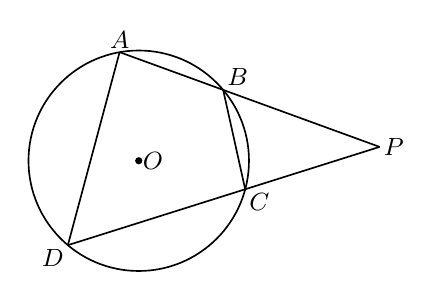
\begin{tikzpicture}[semithick, every node/.style={inner sep=1.2pt, font=\small}]
  \coordinate (O) at (0,0);
  \coordinate (A) at (-0.243,1.379);
  \coordinate (B) at (1.072,0.900);
  \coordinate (C) at (1.352,-0.362);
  \coordinate (D) at (-0.900,-1.072);
  \coordinate (P) at (3.059,0.176);
  \draw (0,0) circle (1.4);
  \fill (O) circle (1.3pt);
  \draw (A) -- (P);
  \draw (D) -- (P);
  \draw (A) -- (D);
  \draw (B) -- (C);
  \node[above] at (A) {$A$};
  \node[above right] at (B) {$B$};
  \node[below right] at (C) {$C$};
  \node[below left] at (D) {$D$};
  \node[right] at (P) {$P$};
  \node[right] at (O) {$O$};
\end{tikzpicture}
\end{center}
\nopagebreak[4]
\Needspace{4\baselineskip}
\textbf{解析}

用圆内接四边形的相似三角形与割线定理。

\Needspace{5\baselineskip}
四边形 $ABCD$ 内接于圆，故 $\angle PBC=\angle PDA$，$\angle PCB=\angle PAD$，于是 $\triangle PBC\sim\triangle PDA$，

\nopagebreak[4]
\[\frac{BC}{AD}=\frac{PB}{PD}=\frac{PC}{PA}.\]

\Needspace{5\baselineskip}
又由割线定理 $PA\cdot PB=PC\cdot PD$。设 $PB=x$，则 $PA=2x$；设 $PC=y$，则 $PD=3y$，于是

\nopagebreak[4]
\[2x^2=3y^2\Longrightarrow \frac yx=\sqrt{\frac23}.\]

\Needspace{5\baselineskip}
故

\nopagebreak[4]
\[\frac{BC}{AD}=\frac{PC}{PA}=\frac{y}{2x}=\frac12\sqrt{\frac23}=\frac{\sqrt6}6.\]

\gkanswer{答案：$\dfrac{\sqrt6}6$。}

\end{answer}
\begin{answer}
\gksolhead{15}{}

\textbf{题目}：

如图，在 $\triangle ABC$ 中，$AD\perp AB$，$\overrightarrow{BC}=\sqrt3\overrightarrow{BD}$，$|\overrightarrow{AD}|=1$，则 $\overrightarrow{AC}\cdot\overrightarrow{AD}=$ $\underline{\qquad}$。
\nopagebreak[4]
\begin{center}% 2010 年天津卷理科第 15 题：三角形 ABC 与点 D（D 在 BC 上，AD⊥AB）。
% 来源 PDF：普通高考/2010/2010天津理.pdf，SHA-256 340aba76699a12f330637f9c682abbc893e03e0e91788287934c0a7e0a3cace9。
% 原页：第 1 页（A3 六栏）第 3 栏中部，书页码 635。
% 重绘依据：B、D、C 共线，A 在 BC 上方，AD⊥AB；D 为 BC 内一点。
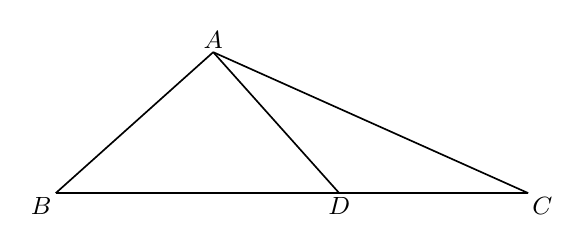
\begin{tikzpicture}[semithick, every node/.style={inner sep=1.2pt, font=\small}]
  \coordinate (B) at (0,0);
  \coordinate (C) at (6,0);
  \coordinate (D) at (3.6,0);
  \coordinate (A) at (2,1.79);
  \draw (B) -- (C);
  \draw (A) -- (B);
  \draw (A) -- (C);
  \draw (A) -- (D);
  \node[above] at (A) {$A$};
  \node[below left] at (B) {$B$};
  \node[below right] at (C) {$C$};
  \node[below] at (D) {$D$};
\end{tikzpicture}
\end{center}
\nopagebreak[4]
\Needspace{4\baselineskip}
\textbf{解析}

以 $A$ 为原点建系，把向量用坐标表示。

\Needspace{5\baselineskip}
取 $A$ 为原点，$\overrightarrow{AD}$ 方向为 $x$ 轴正向，则 $D(1,0)$。由 $AD\perp AB$ 设 $B(0,t)$。由 $\overrightarrow{BC}=\sqrt3\overrightarrow{BD}$ 得

\nopagebreak[4]
\[C=B+\sqrt3(D-B)=(\sqrt3,\ t(1-\sqrt3)).\]

\Needspace{5\baselineskip}
故

\nopagebreak[4]
\[\overrightarrow{AC}\cdot\overrightarrow{AD}=\sqrt3\cdot1+0=\sqrt3.\]

\gkanswer{答案：$\sqrt3$。}

\end{answer}
\begin{answer}
\gksolhead{16}{}

\textbf{题目}：

设函数 $f(x)=x^2-1$，对任意 $x\in\left[\dfrac32,+\infty\right)$，$f\left(\dfrac xm\right)-4m^2f(x)\leqslant f(x-1)+4f(m)$ 恒成立，则实数 $m$ 的取值范围是$\underline{\qquad}$。

\Needspace{4\baselineskip}
\textbf{解析}

把不等式展开，化为关于 $x$ 的二次不等式恒成立问题。

\Needspace{5\baselineskip}
由 $f(x)=x^2-1$ 展开并移项：

\nopagebreak[4]
\[f\left(\frac xm\right)-4m^2f(x)-f(x-1)-4f(m)
=x^2\left(\frac1{m^2}-4m^2-1\right)+2x+3\leqslant0.\]

\Needspace{5\baselineskip}
记 $A=\dfrac1{m^2}-4m^2-1$。若 $A\geqslant0$，$x\to+\infty$ 时左边无界，不成立，故 $A<0$。此时抛物线开口向下，最大值只能在顶点 $x=-\dfrac1A$ 或端点 $x=\dfrac32$ 取得；因 $3-\dfrac1A>3>0$，顶点不能在 $\left[\dfrac32,+\infty\right)$ 内，故只能有

\nopagebreak[4]
\[\frac94A+6\leqslant0\Longrightarrow A\leqslant-\frac83,\]

而此时 $-\dfrac1A\leqslant\dfrac38<\dfrac32$，自洽。

\Needspace{5\baselineskip}
即

\nopagebreak[4]
\[\frac1{m^2}-4m^2+\frac53\leqslant0
\Longrightarrow 12m^4-5m^2-3\geqslant0
\Longrightarrow (4m^2-3)(3m^2+1)\geqslant0.\]

故 $m^2\geqslant\dfrac34$，$m\in\left(-\infty,-\dfrac{\sqrt3}2\right]\cup\left[\dfrac{\sqrt3}2,+\infty\right)$。

\gkanswer{答案：$\left(-\infty,-\dfrac{\sqrt3}2\right]\cup\left[\dfrac{\sqrt3}2,+\infty\right)$。}

\end{answer}
\begin{answer}
\gksolhead{17}{}

\textbf{题目}：

已知函数 $f(x)=2\sqrt3\sin x\cos x+2\cos^2x-1$（$x\in\mathbf R$）。

（1）求函数 $f(x)$ 的最小正周期及在区间 $\left[0,\dfrac\pi2\right]$ 上的最大值和最小值；

（2）若 $f(x_0)=\dfrac65$，$x_0\in\left[\dfrac\pi4,\dfrac\pi2\right]$，求 $\cos2x_0$ 的值。

\Needspace{4\baselineskip}
\textbf{解析}

\Needspace{5\baselineskip}
先把 $f(x)$ 化为一个正弦型函数。

\nopagebreak[4]
\[f(x)=\sqrt3\sin2x+\cos2x=2\sin\left(2x+\frac\pi6\right),\]

\Needspace{5\baselineskip}
故最小正周期 $T=\pi$。当 $x\in\left[0,\dfrac\pi2\right]$ 时，$2x+\dfrac\pi6\in\left[\dfrac\pi6,\dfrac{7\pi}6\right]$，故

\nopagebreak[4]
\[f_{\max}=2\quad\left(x=\frac\pi6\right),\qquad
f_{\min}=-1\quad\left(x=\frac\pi2\right).\]

\Needspace{5\baselineskip}
由 $f(x_0)=\dfrac65$ 得 $\sin\left(2x_0+\dfrac\pi6\right)=\dfrac35$。又 $x_0\in\left[\dfrac\pi4,\dfrac\pi2\right]$，故 $2x_0+\dfrac\pi6\in\left[\dfrac{2\pi}3,\dfrac{7\pi}6\right]$，该区间内正弦为正的部分要求 $2x_0+\dfrac\pi6\in\left[\dfrac{2\pi}3,\pi\right]$，于是

\nopagebreak[4]
\[\cos\left(2x_0+\frac\pi6\right)=-\frac45.\]

\Needspace{5\baselineskip}
所以

\nopagebreak[4]
\[\cos2x_0=\cos\left[\left(2x_0+\frac\pi6\right)-\frac\pi6\right]
=\left(-\frac45\right)\frac{\sqrt3}2+\frac35\cdot\frac12
=\frac{3-4\sqrt3}{10}.\]

\gkanswer{答案：（1）$T=\pi$，最大值 $2$，最小值 $-1$；（2）$\dfrac{3-4\sqrt3}{10}$。}

\end{answer}
\begin{answer}
\gksolhead{18}{}

\textbf{题目}：

某射手每次射击击中目标的概率是 $\dfrac23$，且各次射击的结果互不影响。

（1）假设这名射手射击 $5$ 次，求恰有 $2$ 次击中目标的概率；

（2）假设这名射手射击 $5$ 次，求有 $3$ 次连续击中目标、另外 $2$ 次未击中目标的概率；

（3）假设这名射手射击 $3$ 次，每次射击，击中目标得 $1$ 分，未击中目标得 $0$ 分，在 $3$ 次射击中，若有 $2$ 次连续击中，而另外 $1$ 次未击中，则额外加 $1$ 分；若 $3$ 次全击中，则额外加 $3$ 分。记 $\xi$ 为射手射击 $3$ 次后的总的分数，求 $\xi$ 的分布列。

\Needspace{4\baselineskip}
\textbf{解析}

各次射击相互独立，用二项分布与列举法。

\Needspace{5\baselineskip}
（1）

\nopagebreak[4]
\[P=\mathrm C_5^2\left(\frac23\right)^2\left(\frac13\right)^3
=10\cdot\frac4{243}=\frac{40}{243}.\]

\Needspace{5\baselineskip}
（2）恰有 $3$ 次连续击中且另外 $2$ 次未击中，只有 $HHHMM$、$MHHHM$、$MMHHH$ 三种排列，每种概率为 $\left(\dfrac23\right)^3\left(\dfrac13\right)^2=\dfrac8{243}$，故

\nopagebreak[4]
\[P=3\cdot\frac8{243}=\frac8{81}.\]

（3）三次射击的可能结果为：$HHH$ 得 $3+3=6$ 分；$HHT$、$THH$ 有两次连续击中，得 $2+1=3$ 分；$HTH$ 两次击中不连续，得 $2$ 分；$HTT$、$THT$、$TTH$ 各得 $1$ 分；$TTT$ 得 $0$ 分。故 $\xi$ 的分布列为

\begin{center}
\begin{tabular}{llllll}
\toprule
$\xi$ & $0$ & $1$ & $2$ & $3$ & $6$ \\
\midrule
$P$ & $\dfrac1{27}$ & $\dfrac29$ & $\dfrac4{27}$ & $\dfrac8{27}$ & $\dfrac8{27}$ \\
\bottomrule
\end{tabular}
\end{center}

\gkanswer{答案：（1）$\dfrac{40}{243}$；（2）$\dfrac8{81}$；（3）$P(\xi=0)=\dfrac1{27}$，$P(\xi=1)=\dfrac29$，$P(\xi=2)=\dfrac4{27}$，$P(\xi=3)=\dfrac8{27}$，$P(\xi=6)=\dfrac8{27}$。}

\end{answer}
\begin{answer}
\gksolhead{19}{}

\textbf{题目}：

如图，在长方体 $ABCD-A_1B_1C_1D_1$ 中，$E$、$F$ 分别是棱 $BC$、$CC_1$ 上的点，$CF=AB=2CE$，$AB:AD:AA_1=1:2:4$。

（1）求异面直线 $EF$ 与 $A_1D$ 所成角的余弦值；

（2）证明 $AF\perp$ 平面 $A_1ED$；

（3）求二面角 $A_1-ED-F$ 的正弦值。
\nopagebreak[4]
\begin{center}% 2010 年天津卷理科第 19 题：长方体 ABCD-A1B1C1D1，E、F 分别在 BC、CC1 上。
% 来源 PDF：普通高考/2010/2010天津理.pdf，SHA-256 340aba76699a12f330637f9c682abbc893e03e0e91788287934c0a7e0a3cace9。
% 原页：第 2 页（A3 六栏）第 1 栏下部，书页码 636。
% 重绘依据：AB:AD:AA1=1:2:4，CF=AB=2CE；可见棱实线，被遮挡的 AB、AD、AA1 虚线；
%   另画平面 A1ED 的 A1E、A1D、ED（虚线）与 AF（虚线）、EF（实线）。
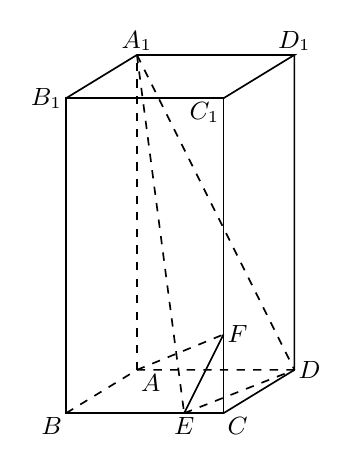
\begin{tikzpicture}[semithick, every node/.style={inner sep=1.2pt, font=\small}]
  \coordinate (B) at (0,0);
  \coordinate (C) at (2,0);
  \coordinate (C1) at (2,4);
  \coordinate (B1) at (0,4);
  \coordinate (A) at (0.9,0.55);
  \coordinate (D) at (2.9,0.55);
  \coordinate (D1) at (2.9,4.55);
  \coordinate (A1) at (0.9,4.55);
  \coordinate (E) at (1.5,0);
  \coordinate (F) at (2,1);
  % 可见棱
  \draw (B) -- (C) -- (C1) -- (B1) -- cycle;
  \draw (B1) -- (A1) -- (D1) -- (C1);
  \draw (D1) -- (D) -- (C);
  % 被遮挡的棱
  \draw[dashed] (B) -- (A) -- (D);
  \draw[dashed] (A) -- (A1);
  % 题设点与辅助线
  \draw (E) -- (F);
  \draw[dashed] (A1) -- (E);
  \draw[dashed] (A1) -- (D);
  \draw[dashed] (E) -- (D);
  \draw[dashed] (A) -- (F);
  \node[above] at (A1) {$A_1$};
  \node[above] at (D1) {$D_1$};
  \node[left] at (B1) {$B_1$};
  \node[below left] at (C1) {$C_1$};
  \node[below left] at (B) {$B$};
  \node[below right] at (C) {$C$};
  \node[right] at (D) {$D$};
  \node[below right] at (A) {$A$};
  \node[below] at (E) {$E$};
  \node[right] at (F) {$F$};
\end{tikzpicture}
\end{center}
\nopagebreak[4]
\Needspace{4\baselineskip}
\textbf{解析}

以 $A$ 为原点建系，用坐标法处理三条问。

\Needspace{5\baselineskip}
设 $AB=1$，则 $AD=2$，$AA_1=4$，$CE=\dfrac12$，$CF=1$。以 $A$ 为原点，$AB$、$AD$、$AA_1$ 为坐标轴建系：

\nopagebreak[4]
\[A(0,0,0),\ B(1,0,0),\ C(1,2,0),\ D(0,2,0),\ A_1(0,0,4),\]
\nopagebreak[4]
\[E\left(1,\frac32,0\right),\ F(1,2,1).\]

\Needspace{5\baselineskip}
（1）

\nopagebreak[4]
\[\overrightarrow{EF}=\left(0,\frac12,1\right),\qquad
\overrightarrow{A_1D}=(0,2,-4).\]

\Needspace{5\baselineskip}
故

\nopagebreak[4]
\[\cos\theta=\frac{\left|\overrightarrow{EF}\cdot\overrightarrow{A_1D}\right|}
{|\overrightarrow{EF}||\overrightarrow{A_1D}|}
=\frac{|-3|}{\frac{\sqrt5}2\cdot2\sqrt5}=\frac35.\]

\Needspace{5\baselineskip}
（2）$\overrightarrow{AF}=(1,2,1)$，而

\nopagebreak[4]
\[\overrightarrow{A_1E}=\left(1,\frac32,-4\right),\qquad
\overrightarrow{ED}=\left(-1,\frac12,0\right),\]

\nopagebreak[4]
\[\overrightarrow{AF}\cdot\overrightarrow{A_1E}=1+3-4=0,\qquad
\overrightarrow{AF}\cdot\overrightarrow{ED}=-1+1+0=0.\]

又 $A_1E$ 与 $ED$ 是平面 $A_1ED$ 内两条相交直线，故 $AF\perp$ 平面 $A_1ED$。

\Needspace{5\baselineskip}
（3）平面 $A_1ED$ 的法向量可取 $\boldsymbol n_1=\overrightarrow{AF}=(1,2,1)$。平面 $DEF$ 中

\nopagebreak[4]
\[\overrightarrow{ED}=\left(-1,\frac12,0\right),\qquad
\overrightarrow{EF}=\left(0,\frac12,1\right),\]

\Needspace{5\baselineskip}
取 $\boldsymbol n_2=(1,2,-1)$。于是

\nopagebreak[4]
\[\cos\langle\boldsymbol n_1,\boldsymbol n_2\rangle
=\frac{1+4-1}{\sqrt6\cdot\sqrt6}=\frac23,\]

故二面角的正弦值为 $\sqrt{1-\dfrac49}=\dfrac{\sqrt5}3$。

\gkanswer{答案：（1）$\dfrac35$；（2）证明；（3）$\dfrac{\sqrt5}3$。}

\end{answer}
\begin{answer}
\gksolhead{20}{}

\textbf{题目}：

已知椭圆 $\dfrac{x^2}{a^2}+\dfrac{y^2}{b^2}=1$（$a>b>0$）的离心率 $e=\dfrac{\sqrt3}2$，连接椭圆的四个顶点得到的菱形的面积为 $4$。

（1）求椭圆的方程；

（2）设直线 $l$ 与椭圆相交于不同的两点 $A$，$B$。已知点 $A$ 的坐标为 $(-a,0)$，点 $Q(0,y_0)$ 在线段 $AB$ 的垂直平分线上，且 $\overrightarrow{QA}\cdot\overrightarrow{QB}=4$，求 $y_0$ 的值。

\Needspace{4\baselineskip}
\textbf{解析}

先由离心率与菱形面积求椭圆方程，再联立直线与椭圆。

\Needspace{5\baselineskip}
（1）四个顶点构成的菱形面积为 $2ab=4$，故 $ab=2$。又

\nopagebreak[4]
\[e^2=\frac34=1-\frac{b^2}{a^2}\Longrightarrow a=2b,\]

于是 $2b^2=2$，$b=1$，$a=2$，椭圆为 $\dfrac{x^2}4+y^2=1$。

\Needspace{5\baselineskip}
（2）$A(-2,0)$，设 $l$ 的斜率为 $k$，则 $y=k(x+2)$。代入椭圆得

\nopagebreak[4]
\[(1+4k^2)x^2+16k^2x+16k^2-4=0.\]

\Needspace{5\baselineskip}
一根为 $-2$，由韦达定理得另一根

\nopagebreak[4]
\[x_B=\frac{2-8k^2}{1+4k^2},\qquad
y_B=k(x_B+2)=\frac{4k}{1+4k^2}.\]

\Needspace{5\baselineskip}
由 $Q$ 在 $AB$ 的垂直平分线上得 $|QA|=|QB|$，即

\nopagebreak[4]
\[4+y_0^2=x_B^2+(y_0-y_B)^2
\Longrightarrow y_0=\frac{x_B^2+y_B^2-4}{2y_B}
=-\frac{6k}{1+4k^2}.\]

\Needspace{5\baselineskip}
再由 $\overrightarrow{QA}\cdot\overrightarrow{QB}=4$：

\nopagebreak[4]
\[-2x_B-y_0(y_B-y_0)=4
\Longrightarrow y_0^2-y_By_0=2x_B+4.\]

\Needspace{5\baselineskip}
代入 $x_B$、$y_B$、$y_0$ 得

\nopagebreak[4]
\[\frac{60k^2}{(1+4k^2)^2}=\frac8{1+4k^2}
\Longrightarrow 60k^2=8(1+4k^2)
\Longrightarrow k^2=\frac27.\]

\Needspace{5\baselineskip}
于是 $k=\pm\dfrac{\sqrt{14}}7$，

\nopagebreak[4]
\[y_0=-\frac{6k}{1+4k^2}=-\frac{14k}5=\mp\frac{2\sqrt{14}}5,\]

即 $y_0=\pm\dfrac{2\sqrt{14}}5$。

\gkanswer{答案：（1）$\dfrac{x^2}4+y^2=1$；（2）$\pm\dfrac{2\sqrt{14}}5$。}

\end{answer}
\begin{answer}
\gksolhead{21}{}

\textbf{题目}：

已知函数 $f(x)=xe^{-x}$（$x\in\mathbf R$）。

（1）求函数 $f(x)$ 的单调区间和极值；

（2）已知函数 $y=g(x)$ 的图象与函数 $y=f(x)$ 的图象关于直线 $x=1$ 对称，证明：当 $x>1$ 时，$f(x)>g(x)$；

（3）如果 $x_1\neq x_2$，且 $f(x_1)=f(x_2)$，证明：$x_1+x_2>2$。

\Needspace{4\baselineskip}
\textbf{解析}

先求导确定单调性与极值，再用对称性作差证明不等式。

\Needspace{5\baselineskip}
（1）

\nopagebreak[4]
\[f'(x)=\mathrm e^{-x}(1-x),\]

故 $x<1$ 时 $f'>0$，$x>1$ 时 $f'<0$；$f$ 在 $(-\infty,1)$ 上递增，在 $(1,+\infty)$ 上递减，极大值为 $f(1)=\dfrac1{\mathrm e}$。

（2）由对称性 $g(x)=f(2-x)=(2-x)\mathrm e^{x-2}$。

当 $x\geqslant2$ 时，$g(x)\leqslant0<f(x)$。

\Needspace{5\baselineskip}
当 $1<x<2$ 时，令 $t=x-1\in(0,1)$，则 $f(x)>g(x)$ 等价于

\nopagebreak[4]
\[\frac{1+t}{1-t}>\mathrm e^{2t}.\]

\Needspace{5\baselineskip}
两边取对数：

\nopagebreak[4]
\[\ln(1+t)-\ln(1-t)=2\left(t+\frac{t^3}3+\frac{t^5}5+\cdots\right)>2t,\]

故不等式成立。综上，当 $x>1$ 时 $f(x)>g(x)$。

\Needspace{5\baselineskip}
（3）不妨设 $x_1<1<x_2$（$f$ 在 $(-\infty,1)$ 与 $(1,+\infty)$ 上分别严格单调，故 $x_1$、$x_2$ 必分居 $1$ 两侧）。若 $x_1+x_2\leqslant2$，则 $x_2\leqslant2-x_1$，且 $2-x_1>1$。由 $f$ 在 $(1,+\infty)$ 上递减得

\nopagebreak[4]
\[f(x_2)\geqslant f(2-x_1).\]

\Needspace{5\baselineskip}
但由（2）取 $x=2-x_1>1$ 得

\nopagebreak[4]
\[f(2-x_1)>g(2-x_1)=f(x_1),\]

于是 $f(x_2)>f(x_1)$，与 $f(x_1)=f(x_2)$ 矛盾。故 $x_1+x_2>2$。

\gkanswer{答案：（1）$f$ 在 $(-\infty,1)$ 上单调递增，在 $(1,+\infty)$ 上单调递减，极大值 $f(1)=\dfrac1{\mathrm e}$，无极小值；（2）证明；（3）证明。}

\end{answer}
\begin{answer}
\gksolhead{22}{}

\textbf{题目}：

在数列 $\{a_n\}$ 中，$a_1=0$，且对任意 $k\in\mathbf N^*$，$a_{2k-1}$，$a_{2k}$，$a_{2k+1}$ 成等差数列，其公差为 $d_k$。

（1）若 $d_k=2k$，证明 $a_{2k}$，$a_{2k+1}$，$a_{2k+2}$ 成等比数列（$k\in\mathbf N^*$）；

（2）若对任意 $k\in\mathbf N^*$，$a_{2k}$，$a_{2k+1}$，$a_{2k+2}$ 成等比数列，其公比为 $q_k$。

① 设 $q_1\neq1$，证明 $\left\{\dfrac1{q_k-1}\right\}$ 是等差数列；

② 若 $a_2=2$，证明 $\dfrac32<2n-\sum\limits_{k=2}^n\dfrac{k^2}{a_k}\leqslant2$（$n\geqslant2$）。

\Needspace{4\baselineskip}
\textbf{解析}

（1）先由公差累加求出奇数项，再算相邻三项。

\Needspace{5\baselineskip}
由 $d_k=2k$ 得

\nopagebreak[4]
\[a_{2k}=a_{2k-1}+2k,\qquad a_{2k+1}=a_{2k}+2k=a_{2k-1}+4k.\]

\Needspace{5\baselineskip}
于是 $a_{2k+1}-a_{2k-1}=4k$，累加得

\nopagebreak[4]
\[a_{2k-1}=a_1+\sum_{j=1}^{k-1}4j=2k(k-1),\]

\Needspace{5\baselineskip}
从而

\nopagebreak[4]
\[a_{2k}=2k(k-1)+2k=2k^2,\qquad
a_{2k+1}=2k^2+2k=2k(k+1),\]

\nopagebreak[4]
\[a_{2k+2}=2(k+1)^2.\]

\Needspace{5\baselineskip}
故

\nopagebreak[4]
\[\frac{a_{2k+1}}{a_{2k}}=\frac{k+1}k=\frac{a_{2k+2}}{a_{2k+1}},\]

即 $a_{2k}$，$a_{2k+1}$，$a_{2k+2}$ 成等比数列。

（2）① 由等差数列与等比数列的相邻关系推出 $q_k$ 的递推式。

\Needspace{5\baselineskip}
由 $a_{2k-1}$，$a_{2k}$，$a_{2k+1}$ 成等差数列得

\nopagebreak[4]
\[a_{2k+3}=2a_{2k+2}-a_{2k+1}.\]

\Needspace{5\baselineskip}
又 $a_{2k}$，$a_{2k+1}$，$a_{2k+2}$ 成等比数列，公比为 $q_k$，故 $a_{2k+2}=q_ka_{2k+1}$。于是

\nopagebreak[4]
\[q_{k+1}=\frac{a_{2k+3}}{a_{2k+2}}
=\frac{2a_{2k+2}-a_{2k+1}}{a_{2k+2}}
=2-\frac1{q_k}.\]

\Needspace{5\baselineskip}
从而

\nopagebreak[4]
\[\frac1{q_{k+1}-1}=\frac1{1-\frac1{q_k}}
=\frac{q_k}{q_k-1}=1+\frac1{q_k-1}.\]

故 $\left\{\dfrac1{q_k-1}\right\}$ 是公差为 $1$ 的等差数列。

② 由 $a_1=0$，$a_2=2$ 及 $a_1$，$a_2$，$a_3$ 成等差数列得 $a_3=4$，故 $q_1=\dfrac{a_3}{a_2}=2$。由①，$\dfrac1{q_k-1}=1+(k-1)=k$，即 $q_k=\dfrac{k+1}k$。

\Needspace{5\baselineskip}
于是

\nopagebreak[4]
\[\frac{a_{2k+2}}{a_{2k}}=q_k^2=\left(\frac{k+1}k\right)^2,\]

累乘得 $a_{2k}=2k^2$，进而 $a_{2k+1}=q_ka_{2k}=2k(k+1)$。

\Needspace{5\baselineskip}
对偶数下标 $2k$，

\nopagebreak[4]
\[\frac{(2k)^2}{a_{2k}}=\frac{4k^2}{2k^2}=2;\]

\Needspace{5\baselineskip}
对奇数下标 $2k+1$，

\nopagebreak[4]
\[\frac{(2k+1)^2}{a_{2k+1}}
=\frac{(2k+1)^2}{2k(k+1)}
=2+\frac2{(2k+1)^2-1}.\]

\Needspace{5\baselineskip}
记 $K$ 为不超过 $n$ 的最大奇数，则

\nopagebreak[4]
\[\sum_{k=2}^n\frac{k^2}{a_k}
=2(n-1)+\sum_{\substack{3\leqslant k\leqslant n\\ k\ \text{\text{奇}}}}\left(\frac1{k-1}-\frac1{k+1}\right)
=2(n-1)+\frac12-\frac1{K+1}.\]

\Needspace{5\baselineskip}
故

\nopagebreak[4]
\[2n-\sum_{k=2}^n\frac{k^2}{a_k}
=\frac32+\frac1{K+1}.\]

\Needspace{5\baselineskip}
当 $n=2$ 时该式为 $2$；当 $n\geqslant3$ 时 $K\geqslant3$，$\dfrac1{K+1}\leqslant\dfrac14$，故

\nopagebreak[4]
\[\frac32<2n-\sum_{k=2}^n\frac{k^2}{a_k}\leqslant\frac74\leqslant2.\]

综上，$\dfrac32<2n-\sum\limits_{k=2}^n\dfrac{k^2}{a_k}\leqslant2$（$n\geqslant2$）。

\gkanswer{答案：（1）证明；（2）① 证明；② 证明。}

\end{answer}